\documentclass[border=10pt]{standalone}

\usepackage{tikz}
\usepackage{tikzsymbols}
\usetikzlibrary{calc,patterns,shapes.geometric}

\def\centerarc[#1](#2)(#3:#4:#5){\draw[#1] ($(#2)+({#5*cos(#3)},{#5*sin(#3)})$) arc (#3:#4:#5);}

\begin{document}
	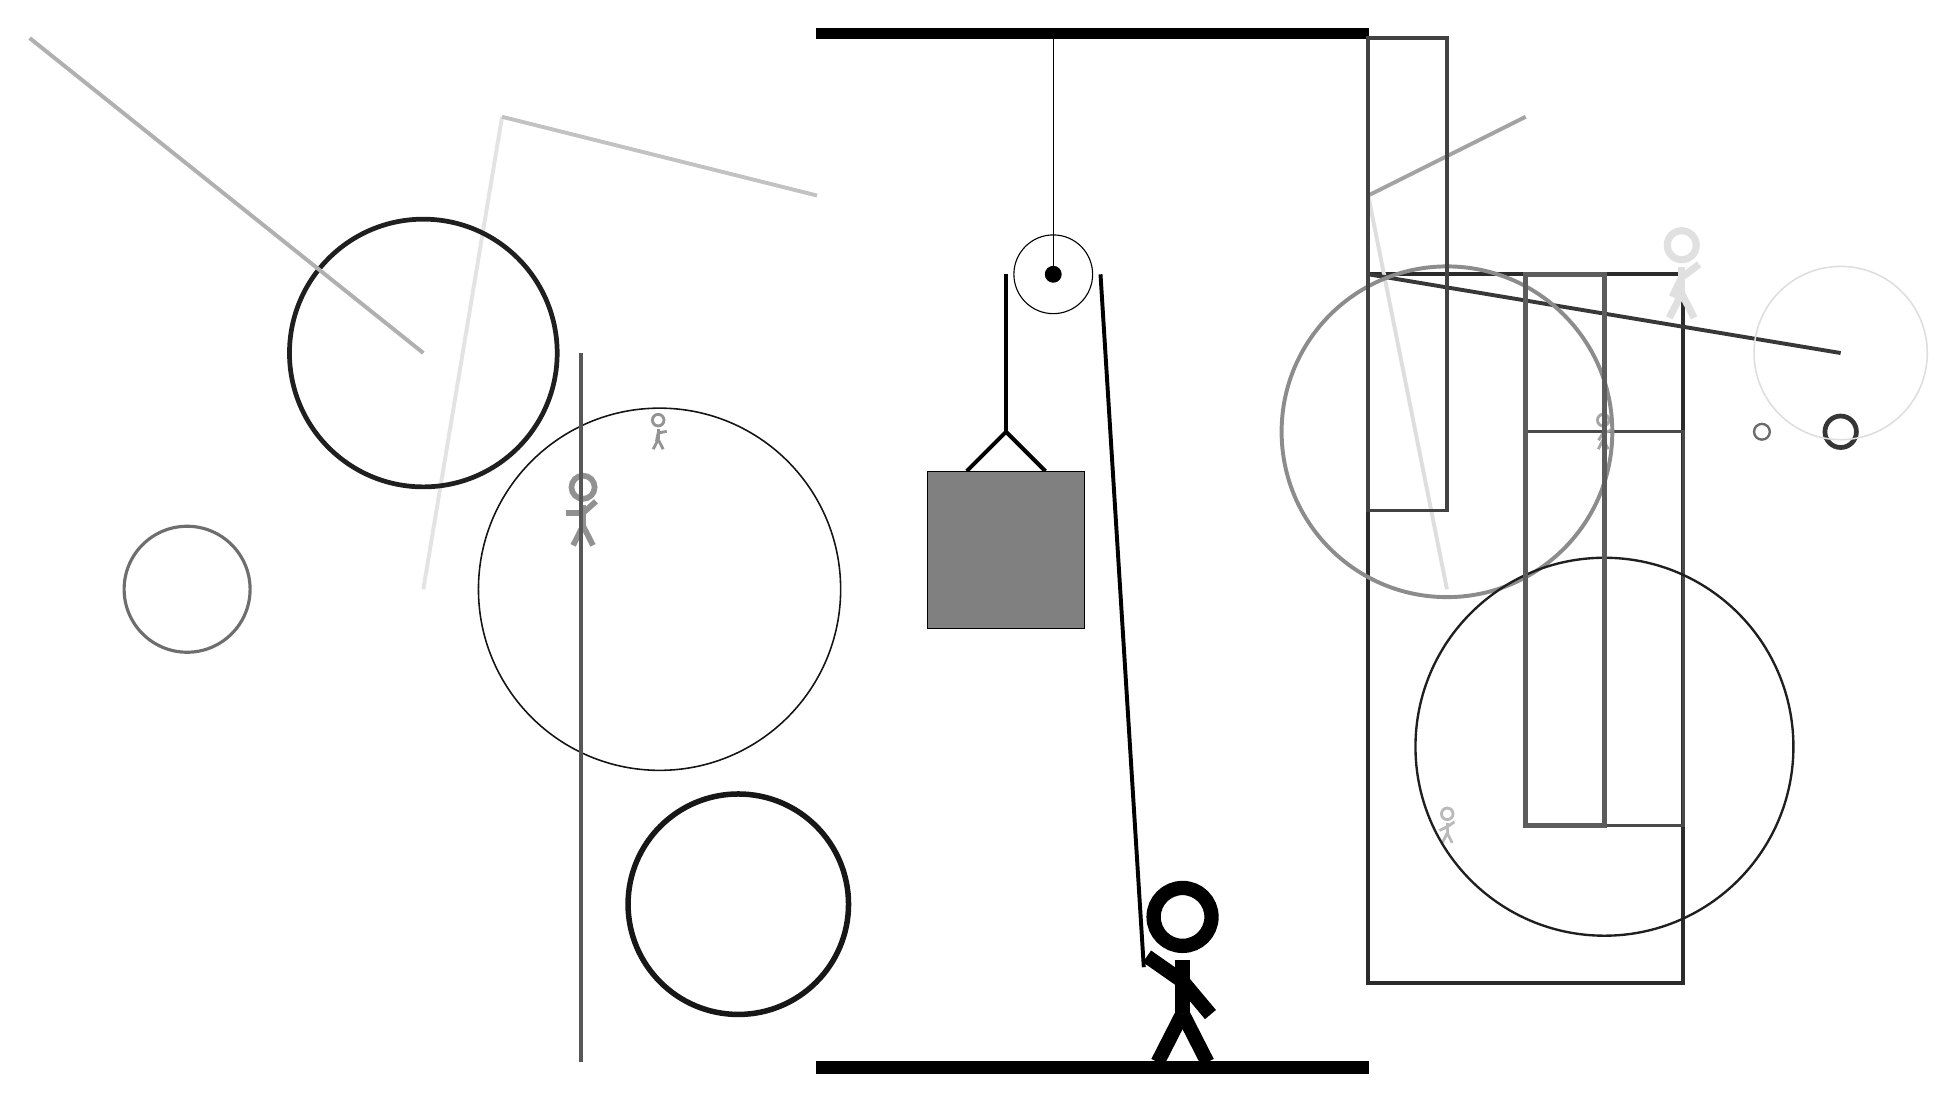
\begin{tikzpicture}
		%%%%% START %%%%%
		
		\draw[fill=black] (-2, 10) rectangle (5, 10.125);
		
		\draw (1, 7) circle (0.5);
		\draw[fill=black] (1, 7) circle (0.1);
		\draw (1, 10) -- (1, 7);
		
		\draw[line width=0.5mm] (-0.1, 4.5) -- (0.4, 5.0) -- (0.9, 4.5);
		\draw[fill=black!50] (-0.6, 4.5) rectangle (1.4, 2.5);
		
		\draw[line width=0.5mm] (0.4, 7) -- (0.4, 5.0);
		\centerarc[line width=0.5mm](1, 7)(0:180:0.6);
		\draw[line width=0.5mm](1.6, 7) -- (2.15, -1.8);
		
		\draw [line width=0.6mm, color=black!79](11, 5) circle (0.2);
		
		\draw[line width=0.5mm, color=black!11](-7, 3) -- (-6, 9);
		\draw[line width=0.5mm, color=black!36](7, 9) -- (5, 8);
		\node[line width=0.4mm, color=black!42] at (-4, 5) {\Strichmaxerl[2][78][11]};
		\draw [line width=0.6mm, color=black!88](-7, 6) circle (1.7);
		\draw[line width=0.5mm, color=black!83] (5, 7) rectangle (9, -2);
		
		\node[line width=0.7mm, color=black!12] at (9, 7) {\Strichmaxerl[5][64][37]};
		
		\draw[line width=0.5mm, color=black!31](-7, 6) -- (-12, 10);
		\node[line width=0.3mm, color=black!43] at (-5, 4) {\Strichmaxerl[4][0][42]};
		\draw [line width=0.2mm, color=black!92](-4, 3) circle (2.3);
		\draw[line width=0.4mm, color=black!71] (7, 0) rectangle (9, 5);
		
		\draw[line width=0.5mm, color=black!13](5, 8) -- (6, 3);
		\draw [line width=0.3mm, color=black!58](10, 5) circle (0.1);
		
		\node[line width=0.6mm, color=black!35] at (8, 5) {\Strichmaxerl[2][57][19]};
		\node[line width=0.6mm, color=black!27] at (6, 0) {\Strichmaxerl[2][26][34]};
		\draw[line width=0.5mm, color=black!78](5, 7) -- (11, 6);
		
		\draw [line width=0.5mm, color=black!45](6, 5) circle (2.1);
		\draw [line width=0.3mm, color=black!88](8, 1) circle (2.4);
		\draw [line width=0.7mm, color=black!91](-3, -1) circle (1.4);
		\draw[line width=0.5mm, color=black!24](-2, 8) -- (-6, 9);
		\draw[line width=0.6mm, color=black!64] (7, 7) rectangle (8, 0);
		
		\draw [line width=0.2mm, color=black!13](11, 6) circle (1.1);
		
		\draw[line width=0.5mm, color=black!66](-5, 6) -- (-5, -3);
		\draw [line width=0.4mm, color=black!57](-10, 3) circle (0.8);
		\draw[line width=0.5mm, color=black!74] (6, 10) rectangle (5, 4);
		
		\node at (2.6, -1.9) {\Strichmaxerl[10][-35][-50]};
		
		\draw[fill=black] (-2, -3) rectangle (5, -3.15);
		
		%%%%% END %%%%%
	\end{tikzpicture}
\end{document}